\documentclass[a4paper,titlepage]{scrartcl}
\pagestyle{plain}
\usepackage[utf8]{inputenc}
\usepackage[T1]{fontenc}
\usepackage[german]{babel}
\usepackage{units}
\usepackage{amsmath,amssymb,amstext}
\usepackage{pgfplots,pgfplotstable}
\usepackage{numprint}
\usepackage{graphicx}
\usepackage{subcaption}
\usepackage{floatrow}
\floatsetup[table]{capposition=top}

\newfloatcommand{capbtabbox}{table}[][\FBwidth]
\numberwithin{equation}{section}

\title{Auswertung vom Versuch P2-53: Franck-Hertz-Versuch}
\author{Gruppe Di-22\\Jonas Müller, Genti Saliu}
\date{16. Mai 2014}

\begin{document}

\begin{titlepage}
\maketitle
\thispagestyle{empty}
\end{titlepage}

\newpage
\pagenumbering{roman}
\tableofcontents

\newpage
\pagenumbering{arabic}

\section{Einführende Versuche}
\subsection{Energie der neidrigsten Anregung von Quecksilber, Kontaktspannung zwischen Kathode und Anode}
In diesem Versuch sollten anhand einigen aus oszillographischen Beobachtungen entstandenen Franck-Hertz-Kurven die niedrigste beobachtbare Anregung von Quecksilber und die Kontaktspannung zwischen Kathode und Anode bestimmt werden.\\ \\
Die Franck-Hertz-Kurve entsteht, indem man die gemessene Spannung $U_A$ am Auffangsschirm über die Beschleunigungsspannung $U_2$ aufträgt. Dazu schlossen wir also einen Oszilloskopeingang mit $U_A$ und den anderen mit $U_2$ im Franck-Hertz-Aufbau.\\ \\
Bei Veränderung der Kathodenspannung und Spannung $U_1$ können mehr Elektronen für die gleiche Spannung $U_2$ beschleunigt werden, die Franck-Hertz-Kurve wird steiler. $U_1$ verringert die Raumladung in der Nähe der Kathode. Die Raumladung ist eine geladene Wolke um die Kathode herum, die entsteht, wenn Elektronen aus der Kathode austreten.\\ \\
Bei Veränderung der Gegenfeldspannung $U_3$ beeinflusst man, wie stark das Gegenfeld auf die Elektronen wirkt und damit wie viele Elektrone den Auffangschirm erreichen, damit kann man also die Höhe der Franck-Hertz-Peaks einstellen (Betrag von $U_A$).\\ \\
Die Kurven haben wir für verscheidene Temperaturen ($\unit[170]{^{\circ} C}$, $\unit[160]{^{\circ} C}$, $\unit[150]{^{\circ} C}$, $\unit[140]{^{\circ} C}$, $\unit[120]{^{\circ} C}$) aufgenommen und jedes Mal die verschiedenen Spannungsparameter $U_1$ (Spannung zum Transport der Elektronen in der ersten Gitteranode) und $U_3$ (Gegenfeldspannung) so angepasst, dass wir geeignete Franck-Hertz-Kurven mit erkennbaren Peaks aufnehmen konnten. Wir haben ausserdem verschiedene Spannungsformen (Sägezahn- und Rampenspannung) ausprobiert und dabei festgestellt, dass wir mit Sägezahnspannung die besseren Franck-Hertz-Kurven erhielten.\\ \\
\textbf{Die Anregungsenergie} bestimmt man aus dem Durchschnitt der Abständen $\Delta U$ zwischen den Peaks.\\
\textbf{Die Kontaktspannung $U_K$} ermitteln wir:
\begin{equation*}
U_K=n \cdot \overline{\Delta U} - U_2 - U_1
\end{equation*}
wobei $n$ ein Peak und $U_{1}$ bzw. $U_2$ die am Gitter $g_1$ angelegte Spannung und Beschleunigungsspannung sind. Um einen Wert für die Kontaktspannung zu erhalten, bestimmten wir anschliessend den Mittelwert aus diesen Werten.\\ \\
Bei der Berechnung aus den Peaks achteten wir darauf, bei zu großen Abweichungen der Kontaktspannungen etwaige unsichtbare Peaks zu berücksichtigen, um dann bessere Werte zu erhalten. Die Spalte $n$ der Tabelle \ref{tab:aufgabe12} zeigt, ab welchem Peak wir zu zählen anfingen.
\begin{table}[H]
\caption{Anregungsenergien und Kontaktspannungen für verschiedene Temperaturen}
\begin{tabular}{c|c|c|c|c}
	$n$ & $U_1 (V)$ & Temperatur $T (^{\circ} C)$ & Anregungsenergie $\overline{E} (eV)$ & Kontaktspannung $U_K (V)$ \\
	\hline
	2 & 4.3 & 172 & 4.85 & -3.36 \\
	2 & 3.88 & 160 & 5.05 & -2.35 \\
	2 & 3.45 & 150 & 5.21 & -1.98 \\
	2 & 2.59 & 140 & 5.48 & -1.57 \\
	1 & 1.23 & 120 & 5.28 & -3.00 \\
\end{tabular}
\label{tab:aufgabe12}
\end{table}

Auffallend bei der Auswertung der Messdaten ist, dass die ermittelte Anregungsenergie mit steigender Temperatur dem Literaturwert ($\unit[4.89]{eV}$) näher kommt. Bei höheren Temperaturen waren die Peaks schärfer zu erkennen.\\ \\
Es scheint anhand unserer Ergebnisse keine offensichtliche Abhängigkeit der Thermokontaktspannung $U_K$ von der Temperatur vorhanden zu sein, obwohl die temperaturabhängige Thermospannung da ihren Beitrag liefert. Die große Varianz zwischen den Werten könnte an unseren Messdaten liegen.

\begin{figure}[H]
	\centering
	\begin{tabular}{@{}r@{}}
	    \begin{subfigure}[b]{0.48\textwidth}
	    	\centering
			\includegraphics[width=\textwidth]{bilder/Aufgabe1.2/120grad.png}
			\caption{Bei $T = \unit[120]{^{\circ}C}$}
			\label{fig:airInductor300}
		\end{subfigure}
		
	    \begin{subfigure}[b]{0.48\textwidth}
	    	\centering
			\includegraphics[width=\textwidth]{bilder/Aufgabe1.2/140grad.png}
			\caption{Bei $T = \unit[140]{^{\circ}C}$}
			\label{fig:airInductor30}
		\end{subfigure}\\
		
	    \begin{subfigure}[b]{0.48\textwidth}
	    	\centering
			\includegraphics[width=\textwidth]{bilder/Aufgabe1.2/150grad.png}
			\caption{Bei $T = \unit[150]{^{\circ}C}$}
			\label{fig:airInductor30}
		\end{subfigure}
		
	    \begin{subfigure}[b]{0.48\textwidth}
	    	\centering
			\includegraphics[width=\textwidth]{bilder/Aufgabe1.2/160grad.png}
			\caption{Bei $T = \unit[160]{^{\circ}C}$}
			\label{fig:airInductor30}
		\end{subfigure}\\
		
	    \begin{subfigure}[b]{0.48\textwidth}
	    	\centering
			\includegraphics[width=\textwidth]{bilder/Aufgabe1.2/170grad.png}
			\caption{Bei $T = \unit[172]{^{\circ}C}$}
			\label{fig:airInductor30}
		\end{subfigure}
		\footnotesize\sffamily\textbf{Quelle:} Oszilloskop
	\end{tabular}
    \caption{Franck-Hertz-Kurve bei unterschiedlichen Temperaturen}
    \label{fig:franckHertzCurve}
\end{figure}

\subsection{Messung des Anodenstroms}
In diesem Versuch sollte, wie in der Vorbereitung beschrieben, die $U^{\frac{3}{2}}$-Abhängigkeit des (modifizierten) Raumladungsgesetz aus der Vorbereitungshilfe gezeigt werden:

\begin{equation*}
I_{g_2} \approx \lambda U^{\frac{3}{2}}
\end{equation*}

Dazu wird die Gleichung logarithmiert und die Messwerte aufgetragen. Die Spannung wurde in $\unit[2]{V}$-Schritten von $\unit[0]{V}$ bis auf ca. $\unit[31.7]{V}$ (maximal einstellbarer Spannungswert) gesteigert. Als Temperatur in der Röhre wurden $\unit[150]{^\circ C}$ gewählt. Zu dieser Temperatur ist auch die Kontaktspannung bekannt $U_{K}=\unit[-1,98]{V}$, welche zusammen mit der Vorspannung $U_1= \unit[4,3]{V}$ beim Auftragen der Beschleunigungsspannung berücksichtigt werde muss:

\begin{table}[H]
\centering
\caption{Messwerte zur Messung des Anodenstroms}
	\begin{tabular}{c|c|c|c|c}
   $I_{g_2}$ $(\mu A)$ & $\ln{(I_{g_2} (\mu A))}$ & $U_2$ in $V$ (gemessen) & $U$ in $V$ (korrigiert) & $\ln{(U (V))}$ \\
		\hline
		0.05 & -3.00 & 2 & 4.32 & 1.46 \\
        0.10 & -2.30 & 4 & 6.32 & 1.84 \\
	    0.13 & -2.04 & 6 & 8.32 & 2.11 \\
	    0.21 & -1.56 & 8 & 10.32 & 2.33 \\
	    0.26 & -1.35 & 10 & 12.32 & 2.51 \\
	    0.32 & -1.14 & 12 & 14.32 & 2.66 \\
	    0.38 & -0.97 & 14 & 16.32 & 2.79 \\
	    0.44 & -0.82 & 16 & 18.32 & 2.91 \\
	    0.51 & -0.67 & 18 & 20.32 & 3.01 \\
	    0.59 & -0.53 & 20 & 22.32 & 3.11 \\
	    0.67 & -0.40 & 22 & 24.32 & 3.19 \\
	    0.79 & -0.24 & 24 & 26.32 & 3.27 \\
	    0.94 & -0.06 & 26 & 28.32 & 3.34\\
	    1.11 & 0.10 & 28 & 30.32 & 3.41 \\
	    1.40 & 0.34 & 30 & 32.32 & 3.48 \\
	    10.76 & 2.37 & 31.7 & 34.02 & 3.53 \\
	\end{tabular}
\end{table}

\begin{figure}[H]
\centering
\includegraphics[scale=.6]{bilder/aufgabe1.2/regression.png} 
\caption{Lineare Regression zur Messung des Anodenstroms}
\end{figure}

Die lineare Regression mit Mathematica liefert uns eine Steigung von $m_1= 1.67$, was einer Abweichung von $\unit[11]{\%}$ von der erwarteten $U^{\frac{3}{2}}$-Abhängigkeit ist. Allerdings sieht man deutlich, dass das letzte Wertepaar ein Ausreißer ist, ignoriert man dieses beim Fit, so erhält man eine Steigung von $m_2= 1.42$. Dies entspricht nur noch einer Abweichung von $\unit[5.3]{\%}$ darstellt. Insgesamt sind aber beide Werte recht gut, darüber hinaus kann man (bis auf den Ausreißer) sehr deutlich eine lineare Abhängigkeit erkennen.
\subsection{Bestimmung der Ionisierungsarbeit von Quecksilber}
In diesem Versuch sollte die Inonisierungsarbeit von Quecksilber auf zwei verschiedene Arten bestimmt werden. Wir stellten eine Temperatur von $T=\unit[120]{^\circ C}$, eine Spannung $U_1=\unit[1.23]{V}$ und Kathodenspannung $U_K=\unit[5.89]{V}$ ein damit die Elektronen vor den ersten Stößen genügend beschleunigt werden konnten und um so das Gitter $G_1$ als Beschleunigungsgitter zu verwenden.\\

\begin{itemize}
\item \textbf{Anodenstrom in Abhängigkeit von der Anodenspannung}\\ \\
Der Strom wurde hier für verschiedene Spannungen mit einem Multimeter gemessen, wobei wir bei $\unit[0]{V}$ anfingen und dann die Spannung in $\unit[2]{V}$-Schritten steigerten. Wir haben die Werte anschließen aufgetragen und zwei Ausgleichsgeraden gebildet, eine vor und eine nach dem stärksten Anstieg. Die Grenze wurde beim Punkt $(U_2,I_2)=(\unit[24]{V}, \unit[400]{\mu A})$ gezogen (siehe Tabelle mit Messwerten in unserem Protokoll für Aufgabe 1.4).

\begin{figure}[H]
\centering
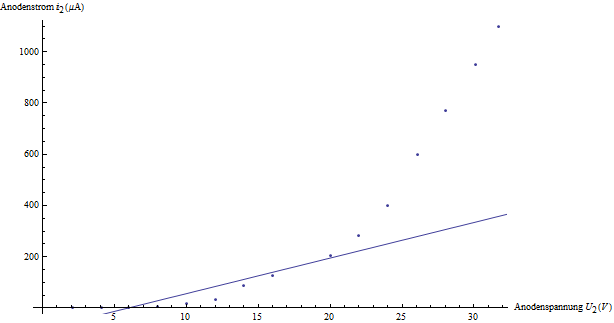
\includegraphics[scale=.7]{bilder/aufgabe1_4a1.png} 
\caption{Anodenstrom $I_2$ über Anodenspannung $U_2$ vor dem stärksten Anstieg}
\end{figure}

\begin{figure}[H]
\centering
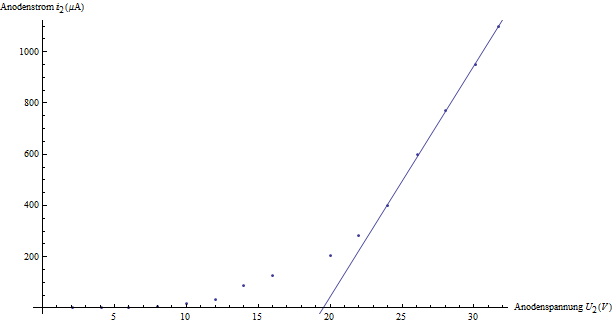
\includegraphics[scale=.7]{bilder/aufgabe1_4a2.png}
\caption{Anodenstrom $I_2$ über Anodenspannung $U_2$ nach dem stärksten Anstieg}
\end{figure}

Der Schnittpunkt dieser Geraden liefert uns für die Ionisierungsarbeit einen Wert von $W_{Ion}= \unit[21,98]{eV}$, korrigiert man den Wert noch mit der Thermokontaktspannung $U_{k}= \unit[-3]{V}$, so erhalten wir $W_{Ion}= \unit[18,98]{eV}$. Dieser Wert weicht leider sehr stark von Literaturwert $W_{Ion,Lit}= \unit[10.44]{eV}$. Dies liegt wohl daran, dass es für uns sehr schwer war ordentliche Werte zu messen, da sich kein wirkliches Gleichgewicht einstellte und der Anodenstrom immer weiter stieg.\\

\item \textbf{Plotten des Auffängerstroms}\\ \\
Bei dieser Methode ließen wir uns vom Oszilloskop den Auffängerstrom (bzw. die am Widerstand abfallende Spannung $U_A$) über die Spannung $U_2$ aufzeichnen. Sobald die Elektronen genügend Energie zu Ionisierung der Atome haben sollte es einen Einbruch des Auffängerstroms gebe. Wir erhielten folgendes Schaubild:

\begin{figure}[H]
\centering
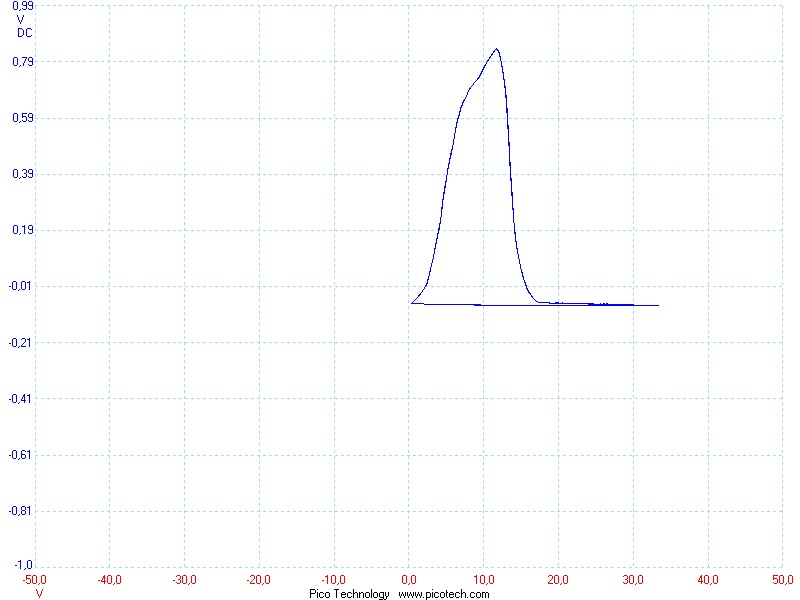
\includegraphics[scale=.4]{bilder/aufgabe1_4_b.jpg}
\caption{$I_A$ über $U_2$} 
\end{figure}

Wir erhielten als Spitzenwert der Spannung $U = \unit[11.77]{V}$ korrigiert man diesen Wert wiederum mit $U_{K}$ so erhalten wir $U_{korr.}=\unit[8.77]{V}$ und für die Ionisierungsarbeit $W_{Ion}=\unit[8.77]{eV}$. Dieser Wert weicht um $\unit[16.0]{\%}$ vom Literaturwert ab. Die relativ große Abweichung könnte an einen schlechten Wert für die Kontaktspannung liegen (siehe oben).\\

\end{itemize}

\subsection{Beobachtung der Emissionslinien bei brennender Gasentladung}
In diesem Versuch haben wir mit einem Taschenspektroskop die Spektralfarben der im Bereich des sichtbaren Lichts liegenden Emissionslinien beobachtet. Mit bloßem Auge waren die Emissionslinen fahlblau.\\ \\
Es war ein Linienspektrum mit den Farben lilla, grün, gelb (orange und rot waren auch zu beobachten, jedoch sind diese dem Glühdraht geschuldet) zu sehen. Die Existenz des Linienspektrums zeigt, dass das Licht des Quecksilbergases bei optischen Übergängen zwischen genau festgelegten angeregten Zuständen der Elektronenhülle entsteht. Diese Beobachtung bestätigt das Bohrsche Atommodell.
\section{Bestimmung der nächsthöheren Anregungsenergie}

Für diesen Versuch wurde ein Aufbau wie in Aufgabe 1.4 verwendet, also $G_1$ als Beschleunigungsgitter verwendet.

\begin{figure}[H]
\centering
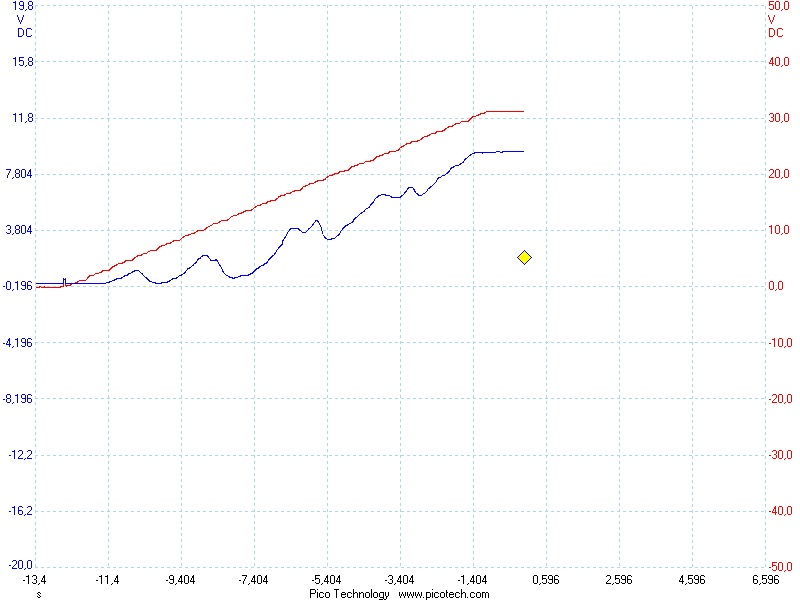
\includegraphics[scale=.4]{bilder/aufgabe2.jpg}
\caption{Höhere Anregungsstufen} 
\end{figure}

Der erste Peak sollte der Energie der ersten Anregungsstufe entsprechen $E_1= \unit[4.89]{eV}$, unsere Messung ergab allerdings eine Wert von $E_{mess}=\unit[5.45]{eV}$, die Differenz dieser Werte kann uns als Offset dienen $U_{off}= \unit[0.56]{V}$. Unsere Messung ergab:

\begin{table}[H]
\centering
\caption{Messwerte bei zweiter Anregungsstufe}
	\begin{tabular}{c|c|c|c}
  Peak & Auffängerspannung $U_A$ in $V$ & $U_2$ in $V$ (gemessen) & $U_B$ in $V$ (korrigiert)\\
		\hline
		1 & 1.009 & 5.45 & 4.89\\
        2 & 2.051 & 10.32 & 9.76\\
        3 & 1.727 & 11.27 & 10.71\\
        4 & 3.994 & 17.19 & 16.63\\
        5 & 4.558 & 18.90 & 18.34\\
        6 & 6.431 & 23.67 & 23.11\\
        7 & 6.905 & 25.87 & 25.31\\
	\end{tabular}
\end{table}

Die Werte für die Peaks können als Linearkombination der Energie der erst und zweiten Anregungsstufe dargestellt werden $p_i= n \cdot U_{1.Anregung} + m \cdot U_{2.Anregung}$, wir wissen, dass $U_{1.Anregung}= \unit[4.89]{V}$ ist. Vergleichen wir unsere Werte damit so können wir n und m bestimmen:

\begin{table}[H]
\centering
\caption{Messwerte bei zweiter Anregungsstufe}
	\begin{tabular}{c|c|c|c|c}
  Peak & n & m & $U_B$ in $V$ (korrigiert) & $ U_{2.Anregung}$ in $V$\\
		\hline
		1 & 1 & 0 & 4.89 & - \\
        2 & 2 & 0 & 9.76 & - \\
        3 & 1 & 1 & 10.71 & 5.82 \\
        4 & 2 & 1 & 16.63 & 6.85 \\
        5 & 1 & 2 & 18.34 & 6.73 \\
        6 & 2 & 2 & 23.11 & 6.67 \\
        7 & 1 & 3 & 25.31 & 6.81 \\
	\end{tabular}
\end{table}

 Damit ergibt sich ein Mittelwert von $\overline{U_{2.Anregung}}=\unit[6.58]{V} $. Dieser Wert weicht nur um $\unit[1,9]{\%}$ vom Literatur Wert $ U_{2.Anregung,Lit}= \unit[6.7]{V}$ ab.
 
 \section{Bestimmung der mittleren Energie der hauptsächlichen Anregung von Neon}
In diesem Versuch sollte die Franck-Hertz-Kurve von Neon untersucht und daraus die mittlere Anregungsenergie von Neon bestimmt werden. Wir beobachteteten qualitativ bei Erhöhung der Beschleunigungsspannung das Auftreten und die Wanderung von Leuchtschichten von der Anode $g_2$ hin zur Kathode. Die Leuchtschichten hatten einen konstanten Abstand voneinander, was sich an dem Weg erklären lässt, den die Elektronen nach einem inelastischen Stoßf durchlaufen mussten um genügend Energie für den nächsten inelastischen Stoß aufzunehmen.\\ \\
Wie in Aufgabe 1.2 haben wir oszillographisch die Entstehung der Franck-Hertz-Kurve und dabei die Peaks der Auffängerschirmspannung beobachtet und den zugehörigen Wert der Beschleunigungsspannung notiert. Wir konnten dabei 4 Peaks feststellen.\\ \\
Für den Abstand zwischen den Peaks erhalten wir:
\begin{table}[H]
\begin{tabular}{c|c|c}
	$U_1 (V)$ & $U_2 (V)$ & $U_3 (V)$ \\
	\hline
	16 & 19 & 17 \\
\end{tabular}
\caption{Anregungsenergien und Kontaktspannungen für verschiedene Temperaturen}
\label{tab:aufgabe3}
\end{table}
Aus dem Mittelwert der Abstände ergibt sich für die mittlere niedrigste Anregungsenergie Folgendes:
\begin{equation}
\overline{E}=\unit[17.33]{eV}
\end{equation}
Der Literaturwert liegt zwischen $\unit[18.5]{V}$ und $\unit[19]{V}$, unsere Messungen müssen nicht sehr genau gewesen und mit großem Fehler behaftet sein.


\section{Bestimmung der mittleren Energie der hauptsächlichen Anregung von Neon}
In diesem Versuch sollte die Franck-Hertz-Kurve von Neon untersucht und daraus die mittlere Anregungsenergie von Neon bestimmt werden. Wir beobachteteten qualitativ bei Erhöhung der Beschleunigungsspannung das Auftreten und die Wanderung von Leuchtschichten von der Anode $g_2$ hin zur Kathode. Die Leuchtschichten hatten einen konstanten Abstand voneinander, was sich an dem Weg erklären lässt, den die Elektronen nach einem inelastischen Stoßf durchlaufen mussten um genügend Energie für den nächsten inelastischen Stoß aufzunehmen.\\ \\
Wie in Aufgabe 1.2 haben wir oszillographisch die Entstehung der Franck-Hertz-Kurve und dabei die Peaks der Auffängerschirmspannung beobachtet und den zugehörigen Wert der Beschleunigungsspannung notiert. Wir konnten dabei 4 Peaks feststellen.\\ \\
Für den Abstand zwischen den Peaks erhalten wir:
\begin{table}[H]
\begin{tabular}{c|c|c}
	$U_1 (V)$ & $U_2 (V)$ & $U_3 (V)$ \\
	\hline
	16 & 19 & 17 \\
\end{tabular}
\caption{Anregungsenergien und Kontaktspannungen für verschiedene Temperaturen}
\label{tab:aufgabe3}
\end{table}
Aus dem Mittelwert der Abstände ergibt sich für die mittlere niedrigste Anregungsenergie Folgendes:
\begin{equation}
\overline{E}=\unit[17.33]{eV}
\end{equation}
Der Literaturwert liegt zwischen $\unit[18.5]{V}$ und $\unit[19]{V}$, unsere Messungen müssen nicht sehr genau gewesen und mit großem Fehler behaftet sein.
\end{document}